\chapter{Background}
\lipsum[1]

\section{Lattice Structure}
\lipsum[1]
\begin{figure}[h]
	\centering
	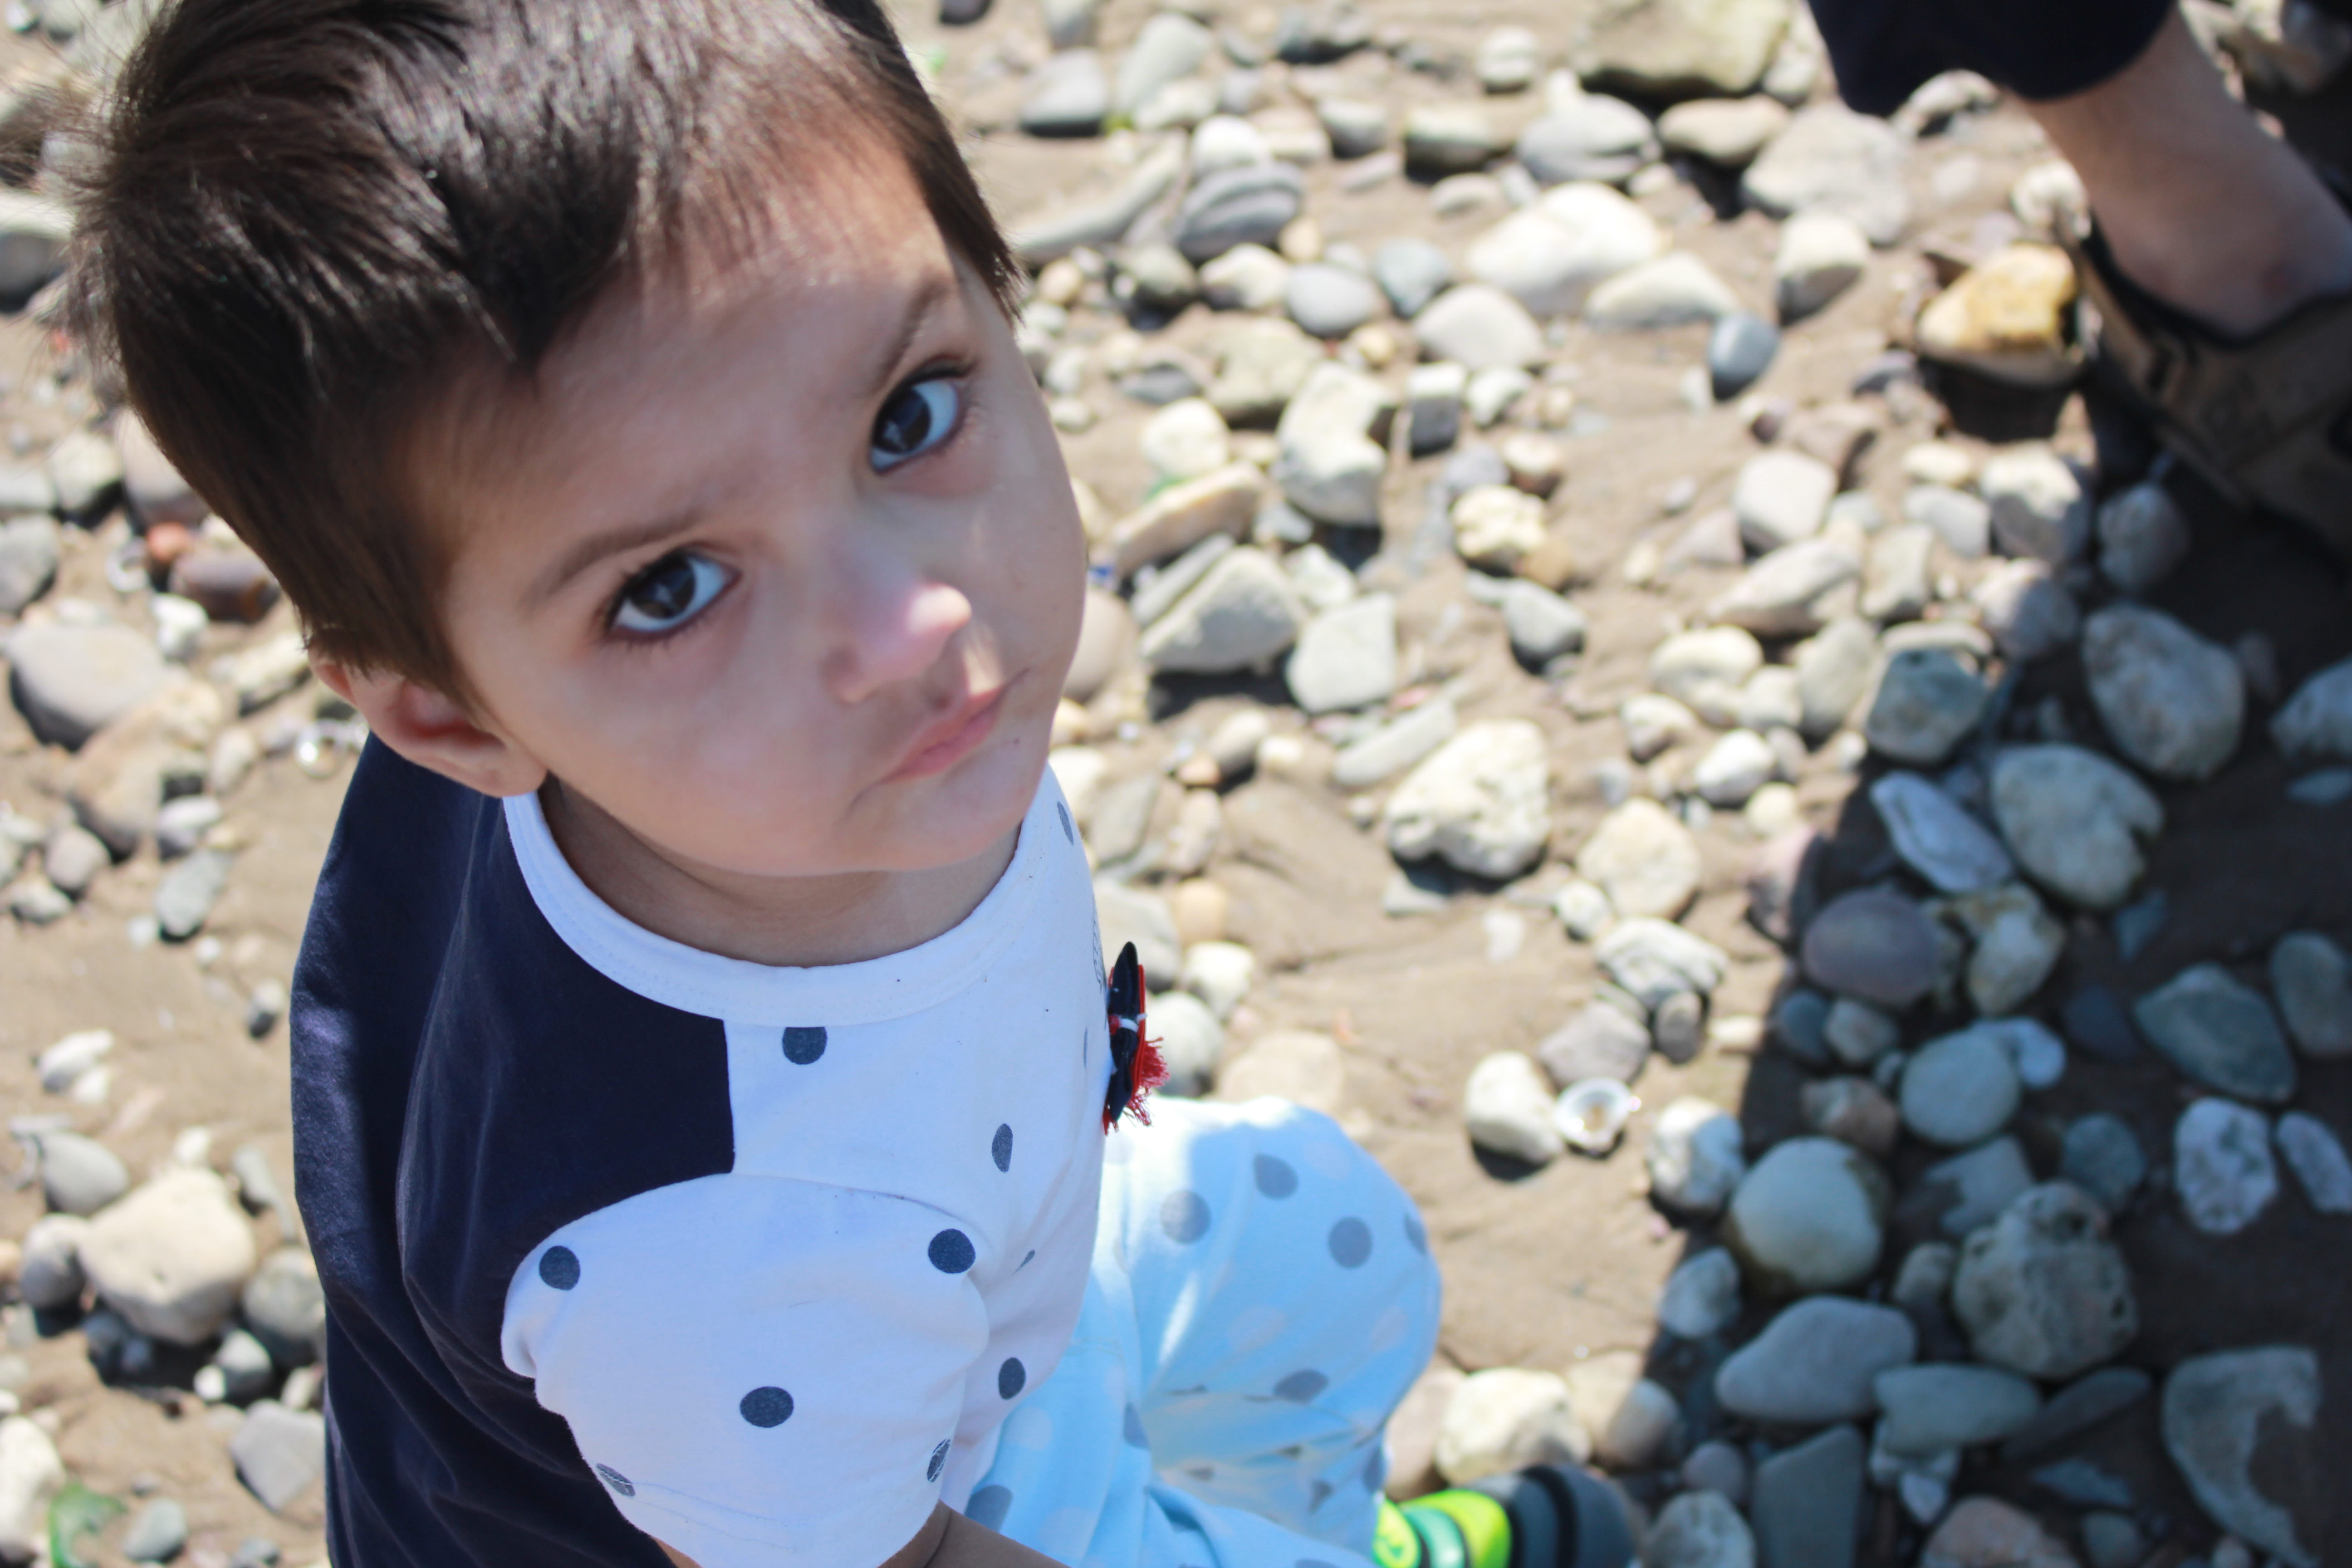
\includegraphics[width=0.7\linewidth]{chapters/chapter1/FiguresCh1/saf2}
	\caption[fig1short]{Long}
	\label{fig:saf2}
\end{figure}

\section{Perodic Table}
at, mollis ac, nulla. Curabitur auctor semper nulla. Donec varius orci eget risus. Duis nibh mi.
\begin{table}[h]
	\caption{First Table}
	\centering
	\begin{tabular}{| c | c | p{4cm} | }
		E11 & E12 & E13 \\ \hline  %END THE ROW first to place a horizontal line
		E21 & E22 & E23 \\
		E31 & E32 & E33 \\
		E41 & E42 & E43 \\
		E51 & E52 & Here I've much longer text, inserted intentionally
	\end{tabular} \\
\end{table}
at, mollis ac, nulla. Curabitur auctor semper nulla. Donec varius orci eget risus. Duis nibh mi

\begin{equation}\label{eq:super1}
E = mc^{(2)}
\end{equation}

\begin{equation}\label{eq:super2}
E = mc^{(2)}
\end{equation}

\begin{equation}\label{eq:super3}
E = mc^{(2)}
\end{equation}

\lipsum[1-20]

